% Copyright 2005-2016 Airbus-EDF-IMACS-Phimeca
% Permission is granted to copy, distribute and/or modify this document
% under the terms of the GNU Free Documentation License, Version 1.2
% or any later version published by the Free Software Foundation;
% with no Invariant Sections, no Front-Cover Texts, and no Back-Cover
% Texts.  A copy of the license is included in the section entitled "GNU
% Free Documentation License".
\renewcommand{\filename}{docUC_RespSurface_PolyChaosDrawings.tex}
\renewcommand{\filetitle}{UC : Draw some usefull graphs associated to a polynomial chaos algorithm : polynomial graphs, comparison graph between numerical samples from the model and the meta-model, ...}

% \HeaderNNIILevel
% \HeaderIILevel
\HeaderIIILevel




The objective of this UC is to provide some graphs usefull after the launch of a polynomial chaos algorithm, as, for example :
\begin{itemize}
\item Graph 1 : the drawings of some members of the 1D polynomial family,
\item Graph 2 : the cloud of points making the comparison between the model values and the meta model ones : if the adequation is perfect, points must be on the first diagonal.
\end{itemize}


Details on response surface approximations may be found in the Reference Guide (\extref{ReferenceGuide}{see files Reference Guide - Step Res. Surf. -- Functional Chaos Expansion and -- Polynomial Chaos Expansion}{responseSurface}).\\
The Use Case takes the example of the Jacobi family.\\

\requirements{
  \begin{description}
  \item[$\bullet$] the distribution of the input random vector : {\itshape inputDistribution}
  \item[type:]  a Distribution
  \item[$\bullet$] the limit state function : {\itshape limitStateFunction}
  \item[type:]   a NumericalMathFunction
  \item[$\bullet$] the meta model : {\itshape metaModel}
  \item[type:] a NumericalMathFunction
  \end{description}
}
             {
               \begin{description}
               \item[$\bullet$] graph described above : {\itshape graphJacobi}
               \item[type:] Graph
               \end{description}
             }


             \textspace\\
             Python  script for this UseCase :

             \inputscript{script_docUC_RespSurface_PolyChaosDrawings1}

             \inputscript{script_docUC_RespSurface_PolyChaosDrawings2}


             \vspace*{0.1cm}

             The example illustrated here below is the beam example described in Eq. (\ref{equatPoutre}), where :
             \begin{itemize}
             \item $E$ follows the Beta($r = 0.9$, $t = 3.2$, $a = 2.8e7$, $b = 4.9e7$) distribution,
             \item $F$ follows the Gamma($k = 3e5$, $\lambda = 9e3$, $\gamma = 1.5e4$)  distribution,
             \item $L$ follows the Uniform($a = 250$, $b=260$) distribution,
             \item $I$ follows the Beta($r = 2.5$, $t = 4.0$, $a = 3.1e2$, $b = 4.5e2$) distribution,
             \item the four components are independent.
             \end{itemize}

             We took the following 1D polynomial families, which parameters have been determined in order to be adapted to the marginal distributions of the input random vector :
             \begin{itemize}
             \item $E$ : Jacobi($\alpha = 1.3$, $\beta = -0.1$, \textit{param}=Jacobi.ANALYSIS),
             \item $F$ : Laguerre($k = 1.78$, Laguerre.ANALYSIS),
             \item $L$ : Legendre,
             \item $I$ : Jacobi($\alpha = 0.5$, $\beta = 1.5$).
             \end{itemize}

             The truncature strategy of the multivariate orthonormal basis is the Cleaning Strategy where we considered within the $500$ first terms of the multivariate basis, among the 50 most significant ones, those which contribution wre significant (which means superior to $10^{-4}$).\\

             The evaluation strategy of the approximation coefficients is the least square strategy based on a design of experiments  determined with the Monte Carlo sampling technique of size 100.\\

             Figures (\ref{PCE_E}) to (\ref{ModelsComparison}) draw the graphs mentioned above.




             \begin{figure}[H]
               \begin{minipage}{9cm}
                 \begin{center}
                   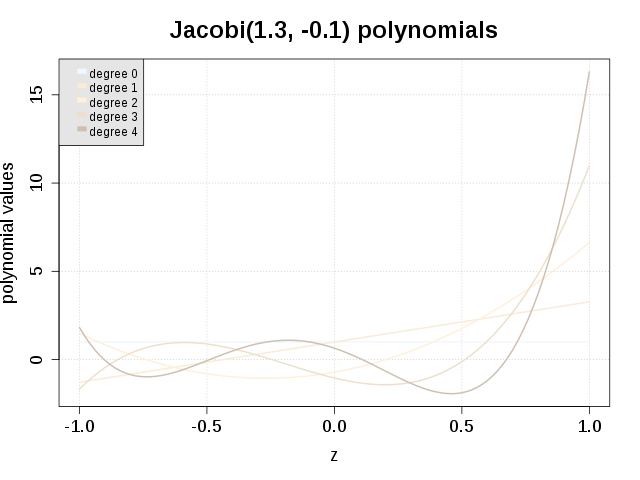
\includegraphics[width=7cm]{Figures/PCE_JacobiPolynomials_VariableE.png}
                   \caption{The 5-th first polynomials of the Jacobi family associated to the variable E.}
                   \label{PCE_E}
                 \end{center}
               \end{minipage}
               \hfill
               \begin{minipage}{9cm}
                 \begin{center}
                   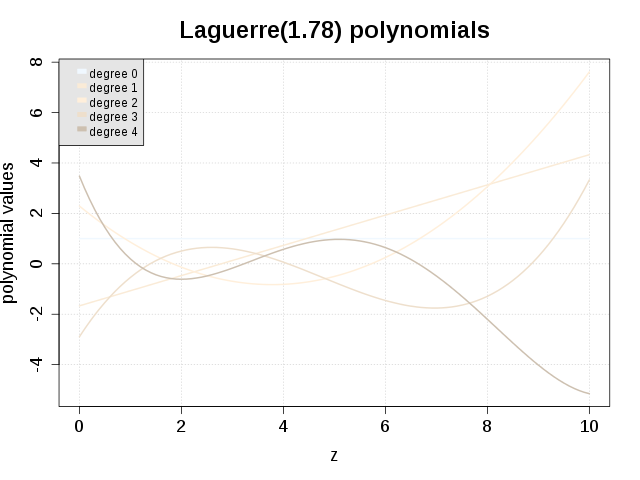
\includegraphics[width=7cm]{Figures/PCE_LaguerrePolynomials_VariableF.png}
                   \caption{The 5-th first polynomials of the Laguerre family associated to the variable F.}
                   \label{PCE_F}
                 \end{center}
               \end{minipage}
             \end{figure}

             \begin{figure}[H]
               \begin{minipage}{9cm}
                 \begin{center}
                   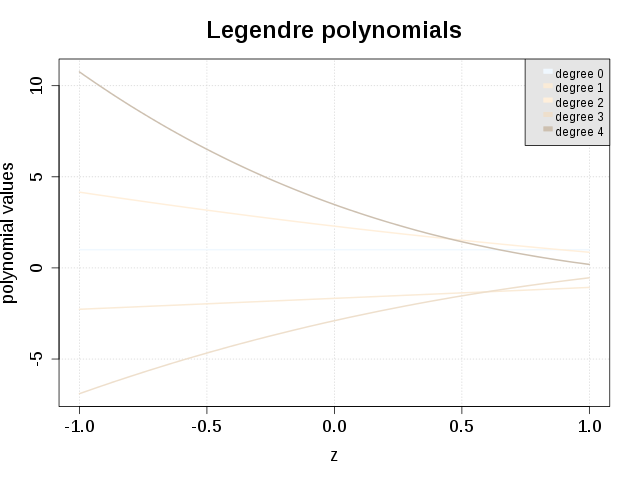
\includegraphics[width=7cm]{Figures/PCE_LegendrePolynomials_VariableL.png}
                   \caption{The 5-th first polynomials of the Legendre associated to the variable I.}
                   \label{PCE_L}
                 \end{center}
               \end{minipage}
               \hfill
               \begin{minipage}{9cm}
                 \begin{center}
                   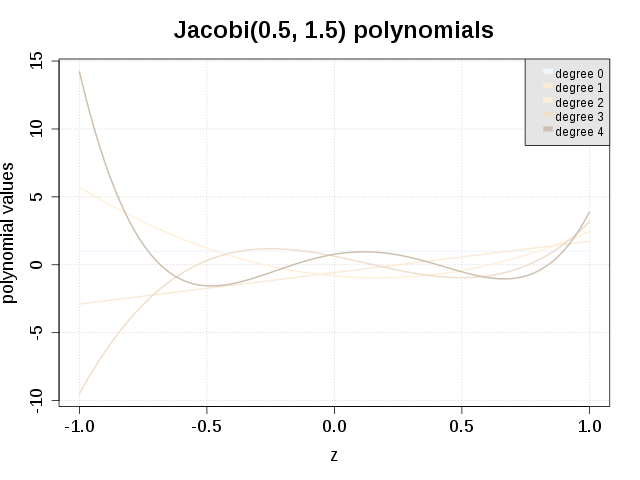
\includegraphics[width=7cm]{Figures/PCE_JacobiPolynomials_VariableI.png}
                   \caption{he 5-th first polynomials of the Jacobi family associated to the variable I.}
                   \label{PCE_I}
                 \end{center}
               \end{minipage}
             \end{figure}




             \begin{figure}[H]
               \begin{center}
                 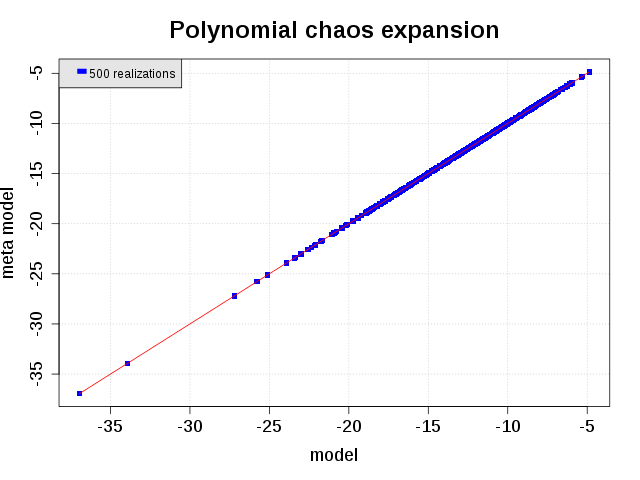
\includegraphics[width=7cm]{Figures/PCE_comparisonModels.png}
                 \caption{Comparison of values from the model and the polynomial chaos meta model.}
                 \label{ModelsComparison}
               \end{center}
             \end{figure}


             Figures (\ref{PCE_Kraw}) to (\ref{PCE_Char}) draw the  5-th first polynomials of the Krawtchouk and Charlier  family respectively associated to the $Binomial(N=5,p=0.6)$ and $Poisson(0.6)$ distributions.



             \begin{figure}[H]
               \begin{minipage}{9cm}
                 \begin{center}
                   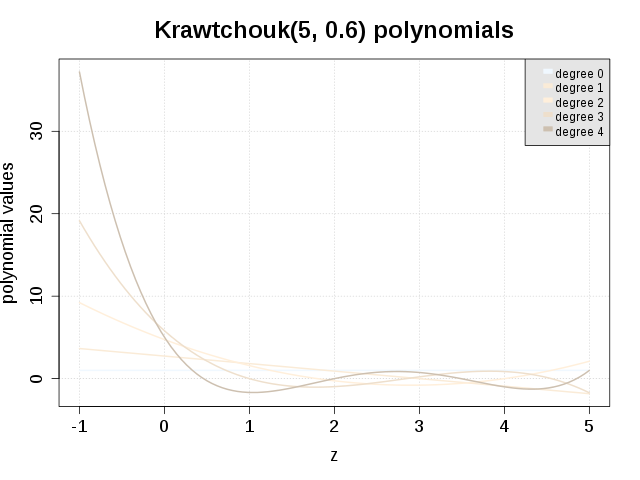
\includegraphics[width=7cm]{Figures/PCE_KrawtchoukPolynomials.png}
                   \caption{The 5-th first polynomials of the Krawtchouk associated to the  $Binomial(N=5,p=0.6)$ measure.}
                   \label{PCE_Kraw}
                 \end{center}
               \end{minipage}
               \hfill
               \begin{minipage}{9cm}
                 \begin{center}
                   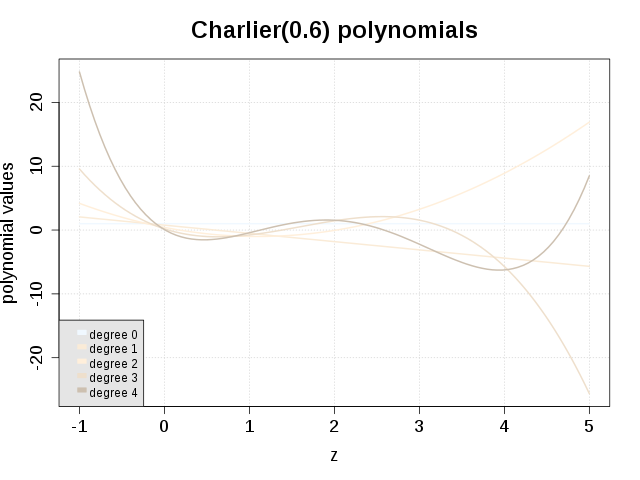
\includegraphics[width=7cm]{Figures/PCE_CharlierPolynomials.png}
                   \caption{The 5-th first polynomials of the Charlier  family associated to the $Poisson(0.6)$ measure.}
                   \label{PCE_Char}
                 \end{center}
               \end{minipage}
             \end{figure}
